\documentclass[SoftwareDesign/SoftwareDesign_main.tex]{subfiles}

\begin{document}
\section{Design af Send Request ViewModel}
Når bruger/lejer har trykket på en bil inde fra SearchView bliver han dirigeret til SendRequest Viewet. Her har SendRequest viewmodel til formål at hente information om bilen, der er blevet trykket på i SearchViewet. Information om bilen bliver sendt med fra SearchViewet, da SendRequest viewmodel har abonneret på en Event Aggregator, som SearchViewModel udsender information til. Informationen vil ved hjælp af databinding blive vist på venstre side af SendRequestViewet. På højre side vil information til udlejer indtastes og herefter sendes til udlejer, hvis informationen er indtastet korrekt. På figur \ref{fig:sendrequestwirefram} ses en wireframe, som designet er gået ud fra. Det endelige resultat varierer dog, da det på venstre side skulle vise lidt mere information end bare et billede.
\begin{figure}[H]
    \centering
    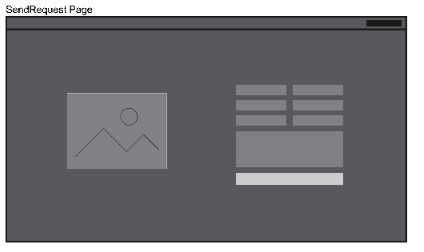
\includegraphics[width=\textwidth]{SoftwareDesign/MVVMDesigns/Graphics/SendRequestWireFrame.PNG}
    \caption{SendRequest WireFrame, som designet tager udgangspunkt i.}
    \label{fig:sendrequestwirefram}
\end{figure}

\subsection{UserControl med databinding}
For at få udskrevet information og tilbehør til bilen er der blevet lavet en UserControl, der ved hjælp af en ContentControl i SendRequestViewet fået sin egen CarProfilModel,der er UserControllens viewmodel.CarProfileModel er en property i SendRequestViewModel, som bliver initialiseret med værdier, når bil information hentes fra databasen. For at vise noget informationen i CarProfileModel til brugeren gøres, der brug af en valueconverter for at vise en boolean værdi i CarProfileModel. Her er true et check ikon og false er et advarsel symbol.
\subsection{Database Interaktion}
Når brugeren navigerer til SendRequest viewet fra SearchViewet skal SendRequest ViewModel udtrække information fra databasen om bilen og udlejeren af bilen. ViewModel bruger herefter denne information til at vise det på skærmen. Når lejeren herefter har indtastet information om ønsket udlejningsdato fra og til, og eventuelt en besked, og trykket "Rent Car", så vil information gemmes i databasen, hvis der ikke er fejl i det indtastede information eller bilen allerede er udlejet i perioden. 
\subsection{Fejlhåndtering}
En vigtig ting i vores applikation er fejlhåndtering, så vi ikke gemmer forkert data i databasen eller information der ikke giver mening. Dette bliver håndteret ved at applikationens tekstbokse og DatePicker controllere bliver røde i kanten og fejlen nævnes i en tooltip. Det er stadig muligt at trykke på knappen "Rent Car". Her vil brugeren i stedet informeres med rød tekst under knappen, hvis information er forkert indtastet. Der bliver også undersøgt om bilen allerede er udlejet i perioden, hvis dette er tilfældet bliver brugeren også informeret med rød skrift.
\subsection{RentCarFunction og kommandoer}
I SendRequestViewModel bruges der en kommando, når knappen "Rent Car" bliver trykket. Efter denne kommando(en prism delegatecommand) bliver triggered, så vil funktionen RentCarFunction kaldes denne funktions ansvar er for det første at tjekke for fejl i tekstbokse og datePickers, hvor funktionen her returnerer med en fejlmeddelelse. Efter dette gøres der brug af en hjælper funktion klasse, hvor funktionen confirmRentingDates bliver kaldt. Denne funktion tjekker på om bilen kan udlejes i den tidsperiode brugeren har indtastet i datepickers. Igen udskrives en fejlmeddelelse, hvis det ikke er muligt. Igen returnere funktionen, hvis ConfirmRentingDates fejler. Hvis funktionen ikke har returneret på dette tidspunkt, så skal information lægges ind i databasen. Der bliver som det næste lavet en liste af de dage, hvor brugeren ønsker at udleje bilen. Herefter bliver informationen lagt ind i databasen for den valgte bil. Udlejer må herefter slette disse dage, hvis han ikke ønsker at udleje til brugeren(lejeren). Dette gøres for at man kan være sikker på at lejer tager stilling til om bilen skal udlejes i perioden. Til dette bliver en hjælper funktion i hjælperklassen igen brugt. Til sidst bliver beskeden lavet og sendt til udlejer(lagt ind i databasen).
\end{document}